\section{Introducción}
\subsection{Sobre mi\ldots}
\begin{frame}{¿Quién soy?}
    \begin{columns}
    \begin{column}{0.75\textwidth}
        \Large
        Benito Palacios Sánchez \\
        \textbf{@pleonex}
    \end{column}
    \begin{column}{0.25\textwidth}
        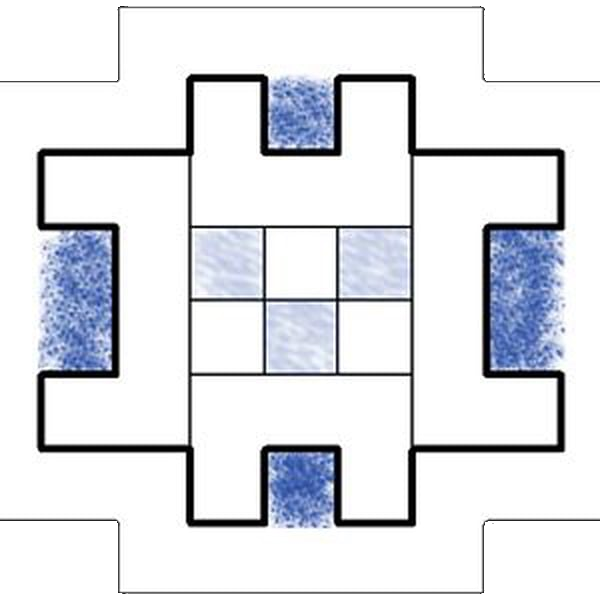
\includegraphics[width=\textwidth]{imgs/pleonex.png}
    \end{column}
    \end{columns}

    \vfill
    \setlength{\leftmargini}{0em}
    \begin{itemize}
        \item<2-> Graduado en Ingeniería de Tecnologías de Telecomunicación
        \begin{itemize}
            \item <2-> Trabajo Fin de Grado sobre seguridad en videojuegos
        \end{itemize}
        \item<3-> Miembro de IEEE Student Branch of Granada
        \item<4-> \textgreater 6 años en el mundo del ROM Hacking
        \item<5-> Miembro de GradienWords
    \end{itemize}
\end{frame}

\subsection{Mis proyectos}
\begin{frame}{Tinke}
    \centering
    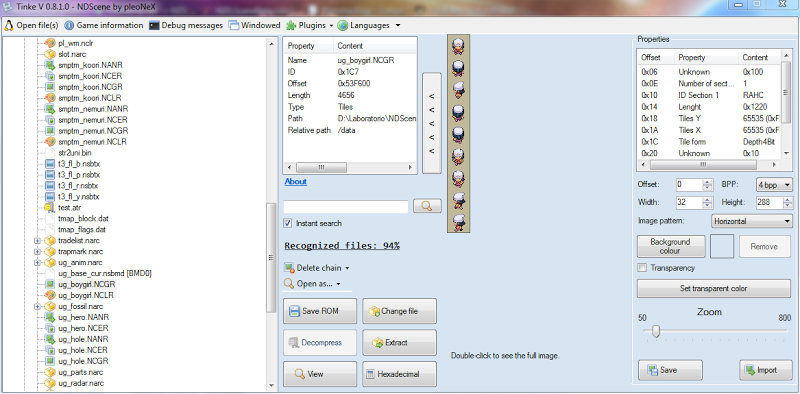
\includegraphics[width=0.65\textwidth]{imgs/tinke_preview.png}
    \vfill
    \includegraphics[width=0.22\textwidth]{imgs/tinke1.png}
    \hfill
    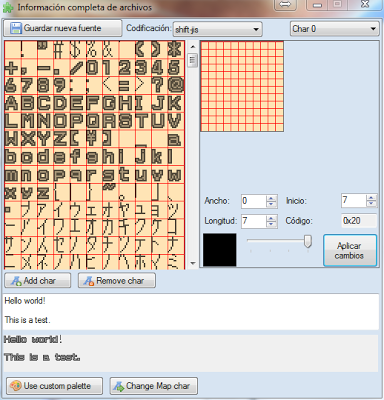
\includegraphics[width=0.22\textwidth]{imgs/tinke2.png}
    \hfill
    \includegraphics[width=0.22\textwidth]{imgs/tinke3.png}
    \hfill
    \includegraphics[width=0.22\textwidth]{imgs/tinke4.png}
\end{frame}

\begin{frame}{Ninokuni: El Mago de las Tinieblas}
    \centering
    \includegraphics[width=0.4\textwidth]{imgs/ninokuni_preview.jpg}
    \vfill
    \includegraphics[width=0.2\textwidth]{imgs/nino1.png}
    \hfill
    \includegraphics[width=0.2\textwidth]{imgs/nino2.png}
    \hfill
    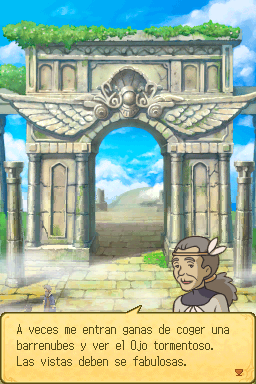
\includegraphics[width=0.2\textwidth]{imgs/nino3.png}
    \hfill
    \includegraphics[width=0.2\textwidth]{imgs/nino4.png}
\end{frame}

\begin{frame}{Fan traducciones}
    \setlength{\leftmargini}{0em}
    \begin{columns}
    \begin{column}{0.5\textwidth}
        \begin{itemize}
            \item<1-> Pokémon Conquest
            \item<2-> Final Fantasy: Four Heroes
        \end{itemize}
        \vfill
        \visible<3->{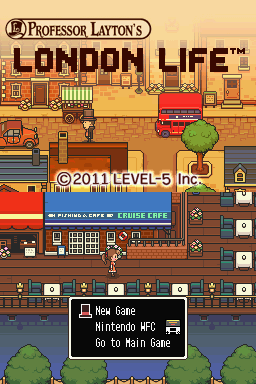
\includegraphics[width=0.4\textwidth]{imgs/london_life.png}}
        \hfill
        \visible<4->{\includegraphics[width=0.4\textwidth]{imgs/sff.png}}
    \end{column}
    \begin{column}{0.5\textwidth}
        \visible<1->{\includegraphics[width=0.4\textwidth]{imgs/pokconquest.png}}
        \hfill
        \visible<2->{\includegraphics[width=0.4\textwidth]{imgs/ff4ol.png}}
        \vfill
        \begin{itemize}
            \item<3-> Profesor Layton: London Life
            \item<4-> Shining Force Feather
        \end{itemize}
    \end{column}
    \end{columns}
\end{frame}

\subsection{El Big Bang}
\begin{frame}{Érase una vez\ldots}
    \centering \includegraphics[width=0.65\textwidth]{imgs/bigbang.jpg}
\end{frame}

\begin{frame}{¿Qué es un fichero?}
    \centering\fontsize{80}{0}\selectfont
    ¿ \includegraphics{imgs/file.png}~?
\end{frame}

\begin{frame}[t]{¿Qué hay dentro de un fichero?}
    \huge\centering
    \uncover<1->{¿Qué hay para que veamos\ldots \\}
    \uncover<2->{\ldots imágenes? \\}
    \uncover<3->{\ldots vídeos? \\}
    \uncover<4->{\ldots música? \\}
    \vfill
    \uncover<5->{¿Cómo lo vemos eso?}
\end{frame}

\begin{frame}{La parte cruda de los archivos}
    \includefigure{BMP visto con editor hexadecimal HxD}{imgs/hexview.png}{0.6}
\end{frame}

\begin{frame}[fragile]{Especificaciones (BMP)}
    \footnotesize
    \ctable[]{ccl}{}{                                                       \FL
        Posición      & Tamaño        & Descripción                         \ML
        \multicolumn{3}{c}{Cabecera estándar}                               \NN
        \texttt{0x00} & \texttt{0x02} & \textit{Magic stamp}: \texttt{BM}   \NN
        \texttt{0x02} & \texttt{0x04} & Tamaño del fichero                  \NN
        \texttt{0x06} & \texttt{0x04} & Reservado                           \NN
        \texttt{0x0A} & \texttt{0x04} & Puntero a los datos de la imagen    \ML
        \multicolumn{3}{c}{Cabecera DIB}                                    \NN
        \texttt{0x00} & \texttt{0x04} & Tamaño de esta cabecera             \NN
        \texttt{0x04} & \texttt{0x04} & Ancho de la imagen                  \NN
        \texttt{0x06} & \texttt{0x04} & Alto de la imagen                   \NN
        \texttt{0x08} & \texttt{0x02} & Número de planos de color (1)       \NN
        \texttt{0x0A} & \texttt{0x02} & Número de bits por píxel            \ML
        \multicolumn{3}{c}{Paleta de colores}                               \ML
        \multicolumn{3}{c}{Píxeles}                                         \LL
    }
\end{frame}

\begin{frame}{Especificaciones (BMP)}
    \begin{columns}
    \begin{column}[T]{0.7\textwidth}
        \begin{tikzpicture}
        \node[anchor=south west,inner sep=0] (image) at (0,0)
        {\includegraphics[width=\textwidth]{imgs/hexview.png}};
            \begin{scope}[x={(image.south east)},y={(image.north west)}]
                \draw<1,6->[red,semithick] (0.15,0.785) rectangle (0.64,0.76);
                \draw<2-5>[red,semithick] (0.15,0.76) rectangle (0.22,0.785);
                \draw<3-5>[red,semithick] (0.22,0.76) rectangle (0.36,0.785);
                \draw<4-5>[red,semithick] (0.36,0.76) rectangle (0.50,0.785);
                \draw<5>[red,semithick] (0.50,0.76) rectangle (0.64,0.785);
                \draw<6,13->[green,semithick] (0.64,0.76) -- (0.64,0.785) -- (0.72,0.785) -- (0.72,0.605) -- (0.50,0.605) -- (0.50,0.58) -- (0.15,0.58) -- (0.15,0.76) -- (0.64,0.76);
                \draw<7-12>[green,semithick] (0.72,0.76) -- (0.64,0.76) -- (0.64,0.785) -- (0.72,0.785);
                \draw<7-12>[green,semithick] (0.15,0.76) -- (0.22,0.76) -- (0.22,0.735) -- (0.15,0.735);
                \draw<8-12>[green,semithick] (0.22,0.735) rectangle (0.36,0.76);
                \draw<9-12>[green,semithick] (0.36,0.735) rectangle (0.50,0.76);
                \draw<10-12>[green,semithick] (0.50,0.735) rectangle (0.57,0.76);
                \draw<11-12>[green,semithick] (0.57,0.735) rectangle (0.64,0.76);
                \draw<12>[green,semithick] (0.64,0.735) -- (0.64,0.76) -- (0.72,0.76) -- (0.72,0.605) -- (0.50,0.605) -- (0.50,0.58) -- (0.15,0.58) -- (0.15,0.735) -- (0.64,0.735);
                \draw<13->[blue,semithick] (0.15,0.12) -- (0.15,0.58) -- (0.50,0.58) -- (0.50,0.605) -- (0.72,0.605) -- (0.72, 0.145) -- (0.50,0.145) -- (0.50,0.12) -- (0.15,0.12);
                \draw<14->[black,semithick] (0.15,0.04) -- (0.15,0.12) -- (0.50,0.12) -- (0.50,0.145) -- (0.72,0.145) -- (0.72,0.04) ;
            \end{scope}
        \end{tikzpicture}
    \end{column}
    \hfill
    \begin{column}[T]{0.4\textwidth}
        \begin{enumerate}
            \item<1-> Cabecera estándar
            \begin{enumerate}
                \item<2-> \textit{Magic stamp}
                \item<3-> Tamaño fichero
                \item<4-> Reservado
                \item<5-> Puntero datos
            \end{enumerate}
            \item<6-> Cabecera DIB
            \begin{enumerate}
                \item<7-> Tamaño DIB
                \item<8-> Ancho
                \item<9-> Alto
                \item<10-> Planos de color
                \item<11-> BPP
                \item<12-> Meta-datos
            \end{enumerate}
            \item<13-> Paleta
            \item<14-> Píxeles
        \end{enumerate}
    \end{column}
    \end{columns}
\end{frame}

\begin{frame}{¿Qué hay dentro de un juego?}
    \fontsize{45}{0}\selectfont
    \begin{columns}
    \begin{column}{0.65\textwidth}
        ¿ \includegraphics{imgs/gamefile.png}~?
        \visible<2->{\textrightarrow}
    \end{column}
    \hfill
    \begin{column}{0.35\textwidth}
        \visible<2->{\includegraphics[width=\textwidth]{imgs/game_desmume.png}}
    \end{column}
    \end{columns}
\end{frame}

\begin{frame}{La parte cruda de un juego}
    \includegraphics[width=\textwidth]{imgs/game_hex.png}
\end{frame}

\begin{frame}{¿Y ahora? ¿Y la especificación?}
    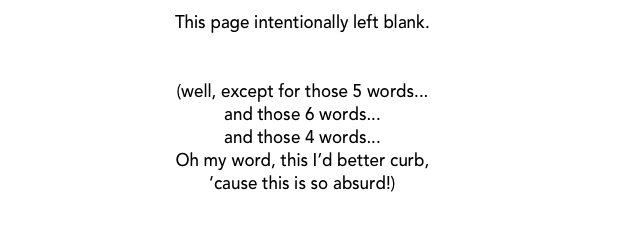
\includegraphics[width=\textwidth]{imgs/left_blank.png}
\end{frame}

\begin{frame}{ROM Hacking}
    \includegraphics[width=\textwidth]{imgs/this_is_romhacking.png}
\end{frame}

\begin{frame}{ROM Hacking}
    \begin{columns}
    \begin{column}{0.35\textwidth}
        Propósito:
        \begin{itemize}
            \item<2-> Fan traducciones
            \item<3-> Mods
            \item<4-> Extraer recursos
            \item<5-> Curiosidad
        \end{itemize}
    \end{column}
    \begin{column}{0.65\textwidth}
        \centering
        \visible<2->{\includegraphics[width=0.45\textwidth]{imgs/ninokuni_preview.jpg}}
        \visible<3->{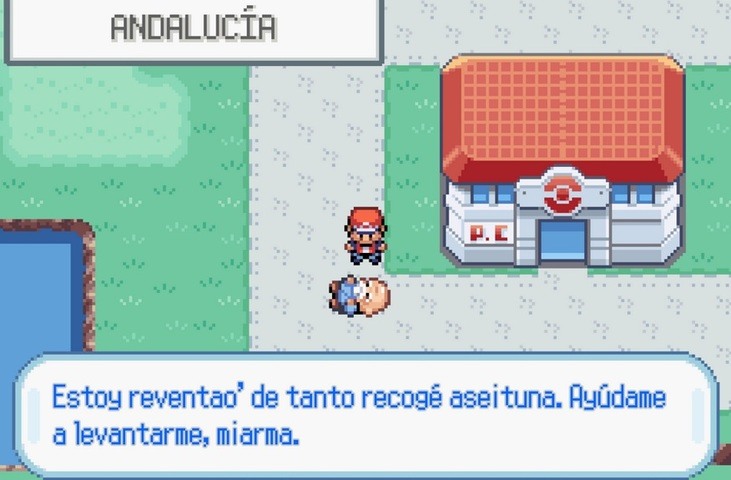
\includegraphics[width=0.45\textwidth]{imgs/mods_preview.jpg}}
        \visible<4->{\includegraphics[width=0.4\textwidth]{imgs/spriters.png}}
        \visible<5->{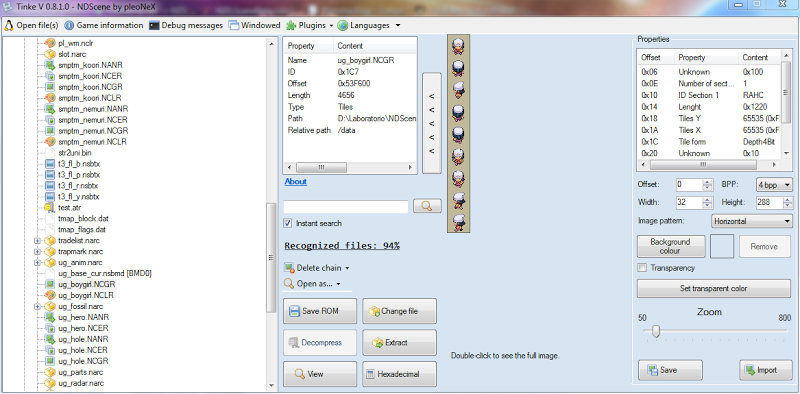
\includegraphics[width=0.8\textwidth]{imgs/tinke_preview.png}}
    \end{column}
    \end{columns}
\end{frame}

\subsection{Temario}
\begin{frame}{Contenido del curso}
    \centering
    \textbf{Introducción al ROM Hacking}

    \begin{enumerate}
        \item<+-> Edita tu primer videojuego
        \begin{enumerate}
            \item ¿Qué es ROM Hacking?
            \item Modifica un videojuego
        \end{enumerate}
        \item<+-> Aprende a editar formatos
        \begin{enumerate}
            \item Textos y tablas
            \item Formatos para imágenes
            \item Audios, tipografías y modelos 3D
        \end{enumerate}
        \item<+-> Programas de edición de videojuegos
        \begin{enumerate}
            \item New Super Mario Bros Level Editor
            \item Super Mario 64 DS Editor
            \item Herramientas de Pokémon (GBA)
            \item Herramientas de Ninokuni
            \note<1>{TileMolester, DSLazy, CUE Compressors}
        \end{enumerate}
    \end{enumerate}
\end{frame}

\begin{frame}<beamer:0|handout:0>{Futuros cursos}
    \begin{columns}
    \begin{column}{0.5\textwidth}
        \uncover<2->{\textbf{Desarrollo de herramientas de ROM Hacking}
        \begin{enumerate}
            \item Crear plugins para Tinke y Libgame.
            \item Crear programas editores de script, imágenes, \ldots
        \end{enumerate}}
    \end{column}
    \hfill
    \begin{column}{0.5\textwidth}
        \uncover<3->{\textbf{ROM Hacking sobre ensamblador}
        \begin{enumerate}
            \item Aprender ensamblador
            \item Depurar juegos
            \item Modificar el código fuente de juegos
        \end{enumerate}}
    \end{column}
    \end{columns}
\end{frame}
